In this section an overview of the system logic and the components which compose it are introduced since they are explain in detail in the following sections. Basically, the platform has been design in a modular way and it is composed of the following modules: State manager, vision, motion and input/output module.

The state manager sets the current state of the robot according to the proximity sensor but mainly based on the information coming from the vision module which directly interacts with the PiCamera. The vision module carries out the analysis of the images being able to segment the scene and extract the position of the sings on the floor. It strongly uses the OpenCV library to perform this task running on the Raspberry Pi. 

\begin{figure}[h!]
     \centering
     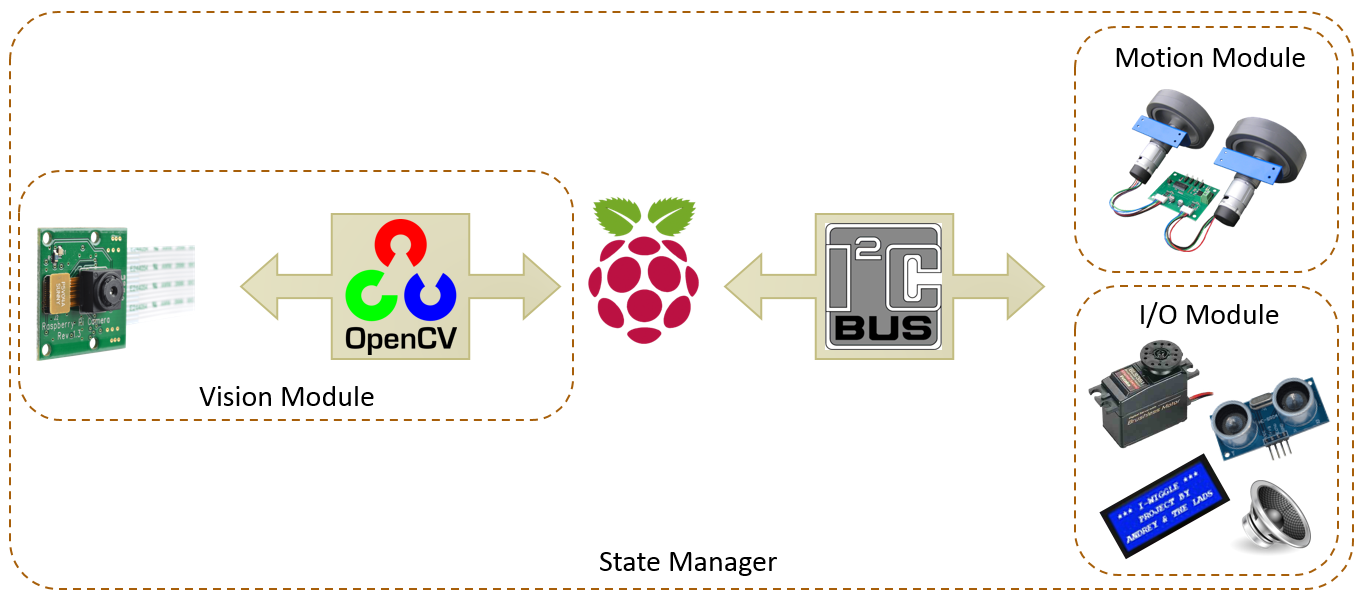
\includegraphics[width=0.7\textwidth]{overview.png}
     \caption{System overview}
     \label{fig:overview}
\end{figure}

Once a sign is detected for instance, the state manager switches the current state acting over the motion module which controls the two motors providing the proper angular and linear speeds. The way both, the motion and the input/output module interact with the board is through the I2C bus enabled in Raspberry Pi.

On the other hand, the input/output module as its name describes, provides visual and sound feedback to the current state of the system enhancing the communication with the user.
